\documentclass{scrartcl}
\usepackage[mathletters]{ucs}
\usepackage[utf8x]{inputenc}
\usepackage{amssymb}
\usepackage{amsmath}
\usepackage[usenames]{color}
\usepackage{hyperref}
\usepackage{wasysym}
\usepackage{graphicx}
\usepackage[normalem]{ulem}
\usepackage{enumerate}

\usepackage{listings}

\lstset{ %
basicstyle=\footnotesize,       % the size of the fonts that are used for the code
showspaces=false,               % show spaces adding particular underscores
showstringspaces=false,         % underline spaces within strings
showtabs=false,                 % show tabs within strings adding particular underscores
frame=single,                   % adds a frame around the code
tabsize=2,                      % sets default tabsize to 2 spaces
breaklines=true,                % sets automatic line breaking
breakatwhitespace=false,        % sets if automatic breaks should only happen at whitespace
}


\title{Second handmade dataset}
\date{dinsdag 08 december 2020}
\author{}

\begin{document}

\maketitle

		\section{Second handmade dataset}

Created vrijdag 13 november 2020



A second handmade dataset is made to compare with the first dataset and get to know what the stripes mean on the \href{./initial_dataset.txt}{first dataset} which was used to measure the wear.



The next setup is used:

The light came primarely from the camera itself which was set in the first brightness setting. 

The camera was located at a distance of 2cm between the housing and the measured point on the insert. The housing starts at the black part; not the plexi glass protector. 

During the making of this dataset the inserts where labeled with bullet or no bullet. This was not setup this way in the first place; instead there was a marker line on the insert. This marker line is also noted in the labels of the dataset.

An "s" means it is with a marker line. A

\begin{tabular}{ |l|l| }
\hline
 symbol & explanation \tabularnewline
\hline
\hline
 s & side with marker line \tabularnewline
\hline
 n & side without marker line \tabularnewline
\hline
 batch number & number specified on the box in which the inserts are kept \tabularnewline
\hline
 plate number & number specified inside the box; this goes from 1 to 10 per batch \tabularnewline
\hline
\end{tabular}


The naming of the dataset is the following

b\_\textless{}batch number\textgreater{}\_p\_\textless{}plate number\textgreater{}\_\textless{}identifier of side\textgreater{}

\href{./Second_handmade_dataset/Second_dataset_setup.tiff}{./Second_handmade_dataset/Second_dataset_setup.tiff}

After looking at the pictures of the datasets it can be confirmed that the 'b' side of the inserts is the side with the mark on. 



This can be seen on the folowing two pictures whis correspond. The first one is from the first dataset, the second from the second dataset.

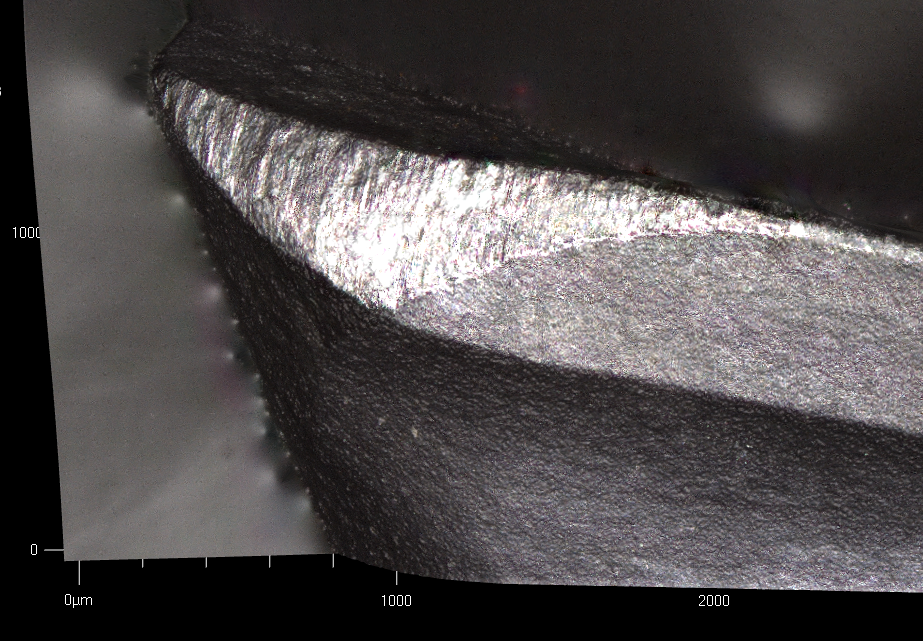
\includegraphics[height=2.083333in, keepaspectratio=true]{./Second_handmade_dataset/t50b-img.PNG}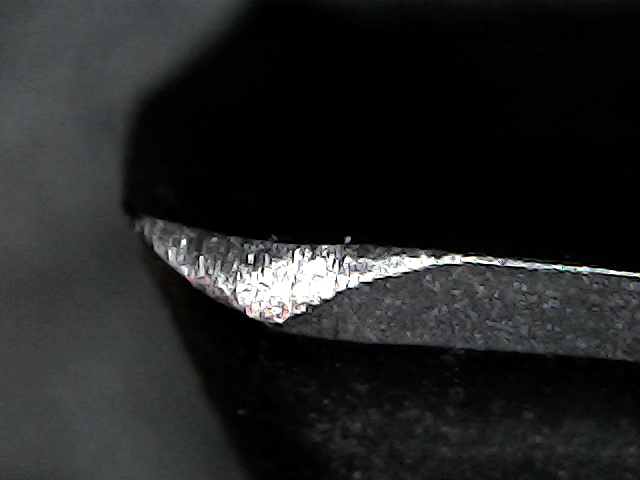
\includegraphics[height=2.083333in, keepaspectratio=true]{./Second_handmade_dataset/b_005_p_010_s.jpg}



\end{document}
